\section{Double zero MVDR ABF}
\label{sec:double-zero-mvdr}
The double zero MVDR (DZ MVDR) ABF is designed to produce broad
beampattern notch in the interferer direction. The DZ MVDR algorithm
exploits the property of the SOZs of array polynomial to produce broad beampattern notches. The flow
diagram \figurename{}~\ref{fig:flow} provides an overview of the DZ
MVDR algorithm. The following section describes the DZ MVDR ABF
algorithm assuming the number of sensors $N$ is odd. The algorithm
extends naturally when $N$ is even by including an additional zero at
$u = 1$ as constrained by even symmetry even length array weights.

\subsection{Algorithm}
\label{sec:algorithm}
The DZ MVDR ABF begins with $L$ data snapshots from an $N$ element
ULA, represented as a data matrix $\dataMat{}$ of dimension
$N \times L$.  The data matrix $\dataMat{}$ is partitioned to create
two submatrices $\dataSubMat{{\rm a}} = \dataMat{(1:K, 1:L)}$ and
$\dataSubMat{\rm b} = \dataMat{(K:N, 1:L)}$ where $K = (N + 1)/2$. The
indices in the subscript of $\dataMat{}$ indicate the range of rows
and columns of $\dataMat{}$ assigned to each submatrix. This
partitioning of the data matrix is equivalent to partitioning the $N$
element full ULA into two $K$ element
subarrays shown in \figurename{}~\ref{fig:subarray}. The $(K-1)\nth$ sensor denoted by white circle is used in both subarrays. The submatrices $\dataSubMat{{\rm a}}$ and
$\dataSubMat{{\rm b}}$ are combined to create an augmented data matrix
$\dataMatK = [\dataSubMat{{\rm a}} | \dataSubMat{{\rm b}}]$ of
dimension $K \times 2L$. The data matrix $\dataMatK$ can be
interpreted as the collection of $2L$ snapshot observed by $K$ element
ULA.

The augmented data matrix is used to compute the subarray sample
covariance matrix
$\sampCov_{\rm K} = (\dataMatK\dataMatK\herm)/(2L)$ and subsequently
the ABF weight vector for a $K$ element subarray
\begin{equation}
  \label{eq:subarray-wt}
  \wtK = \frac{\sampCov_{K}\inv\rep_{K}}{(\rep_{K}\herm \sampCov_{K}\inv\rep_{K})}
\end{equation}
where $\rep_{K}$ is an array manifold vector in the look direction for
the $K$ element subarray. The beamformer in \eqref{eq:subarray-wt} can
be implemented as a SMI MVDR ABF on a $K$ element ULA. The DZ MVDR ABF
weight vector for the full ULA is obtained by convolving the weight vector
$\wtK$ with itself
\begin{equation}
  \label{eq:wt-convo}
  \wtdz = \wtK*\wtK
\end{equation}
where [*] denotes discrete convolution operation considering the weight vector
$\wtK$ as a discrete sequence of length $K$. The resulting DZ MVDR ABF
weight vector $\wtdz$ is of length $2K - 1 = N$.

 The z-transform of \eqref{eq:subarray-wt} yields the array polynomial of
 the subarray SMI MVDR ABF weight vector,
\begin{equation}
  \label{eq:subarray-poly}
  \beampolyz{{\rm K}} = \ztrans{(\wtK)} = G_K\prod_{i=1}^{K - 1}( 1 -
  \sampz_{Ki} z\inv).
\end{equation}
The array polynomial $\beampolyz{{\rm K}}$ has $(K - 1)$ first-order
zeros $\sampz_{Ki}$ on the complex plane. The convolution operation in
\eqref{eq:wt-convo} is equivalent to multiplying the array polynomial
$\beampolyz{{\rm K}}$ with itself to obtain the DZ MVDR array polynomial,
\begin{align*}
\beampolyz{{\rm DZ}} =& \beampolyz{{\rm K}}\beampolyz{{\rm K}} \\
                     =& G_K^2\prod\limits_{i=1}^{K - 1}( 1 -
                        \sampz_{Ki} z\inv)^2  = \ztrans{(\wtdz)}.
\end{align*}
Thus the convolution operation doubles the number of zeros from the
subarray SMI MVDR ABF to produce the DZ MVDR ABF. The DZ MVDR ABF
array polynomial $\beampolyz{{\rm DZ}}$ has $(K - 1)$ SOZs in the same
locations as the zeros of the subarray SMI MVDR ABF. The SOZs produce
broader notches in the beampattern compared to the SMI MVDR ABF.

The DZ MVDR ABF algorithm is extensible to the case when the number of
sensors $N$ is even. When $N$ is even, the subarray size is set to
$K = N/2$. In this case, the convolution operation produces only
$N - 2$ zeros in total while $N - 1$ zeros are required for a $N$
element ULA. The one additional polynomial zero required for the $N$
element ULA weight vector is chosen to be at $z = -1$. This choice is
motivated from the constraint that an FIR filter with a conjugate even
symmetric impulse response and odd number of zeros must have a zero at
$z = -1$ \cite[Sec.~5.7.3]{Oppenheim1989}.

% Algorithm block

\begin{algorithm}
  \caption{DZ MVDR beamformer} \label{alg:dzmvdr}
  \begin{algorithmic}
    \Procedure{SubarrayDataMatrix}{$\dataMat{}$}\Comment{Partition data
    matrix.}
     \State $\dataSubMat{{\rm a}} = \dataMat{1:K,1:L}$
     \State $\dataSubMat{{\rm b}} = \dataMat{K:N,1:L}$
     \State $\dataMatK = \dataSubMat{{\rm a}} | \dataSubMat{{\rm b}}$
    \EndProcedure
    \Procedure{MVDR}{$\dataMatK$}\Comment{Subarray SMI MVDR weights}
    \State $\sampCov_{K} = (\dataMatK \dataMatK\herm)/(2L)$
    \State  $\wtK = \sampCov_{K}\inv\rep_{K}/(\rep_{K}\herm \sampCov_{K}\inv\rep_{K})$
    \EndProcedure
    \Procedure{ConvolveWeights}{$\wtK$}
    \State $\wtdz = \wtK*\wtK$
    \EndProcedure
  \end{algorithmic}
\end{algorithm}


% ------ Flow diagram and sub-array configuration ------
\begin{figure}[!ht]
  \centering

  \subfloat[]
  {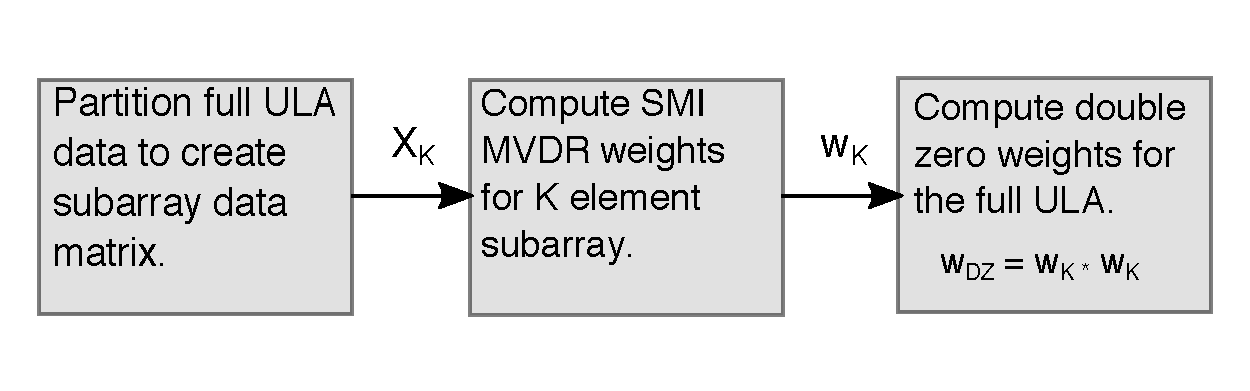
\includegraphics[width=5in]{dz_mvdr_flow.pdf}%
    \label{fig:flow}}
  \vfil

  \subfloat[] 
  {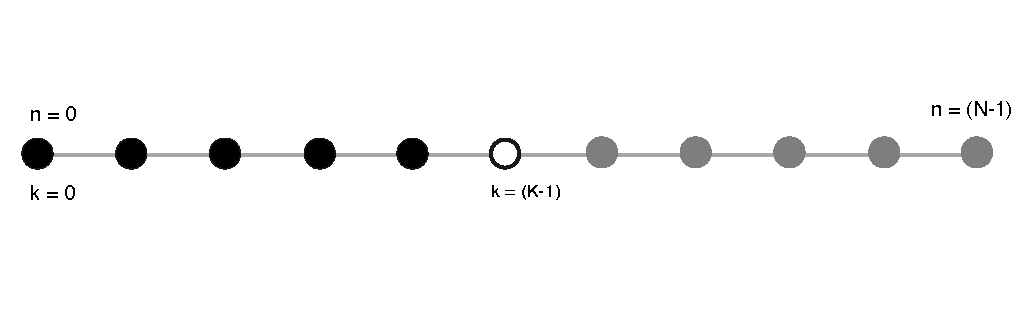
\includegraphics[width=5in]{sub_array.pdf}%
    \label{fig:subarray}}

  \caption{DZ MVDR algorithm (a) flow diagram and (b) two $K$ element
    subarray configuration within the $N$ sensor ULA.}
  \label{fig:dzmvdr}
\end{figure}
% ------------------------------------------------------

The DZ MVDR algorithm involves subarray processing using a $K$ element
subarray. Abraham and Owsley present subarray processing as a
technique to reduce computational overhead for ABFs implemented using
long arrays \cite{abraham89preproc}. The inherent subarray processing
in DZ MVDR ABF also reduces the computational requirement compared to the
standard SMI MVDR ABF implemented on a full ULA saving a factor of 8
in the computation of the SCM inverse. The SCM inversion operation in
\eqref{eq:subarray-wt} takes $\bigO{K^3}$ in contrast to $\bigO{N^3}$
required for the full ULA implementation. Further, the additional
convolution operation in \eqref{eq:wt-convo} takes no more than
$\bigO{K \operatorname{log} K}$. Further, the subarray SCM
($\sampCov_{\rm K}$) is computed using the augmented data matrix with
$2L$ subarray snapshots. The subarray SCM effectively has four times
more snapshots per sensor compared to the standard SCM computed using
the full ULA snapshots. The increase in snapshots to sensor ratio
lowers the bias in the subarray SCM eigenvector estimates which reduces
interferer mismatch \cite{benaych2011eigen, paul2007asymptotics}. The reduction in interferer mismatch enables the DZ MVDR ABF to place deeper notch at the interferer compared to the standard SMI MVDR ABF. 

The computation gain from subarray processing comes at the cost of
reduced spatial degree of freedom (DOF) and widening of the main-lobe
for the DZ MVDR ABF \cite{abraham89preproc}. The DOF is constrained to
about $N/2$, which limits the DZ MVDR ABFs ability to suppress
multiple interferers. Also, the use of $K$ element subarray produces a
main-lobe twice as wide compared to the SMI MVDR ABF using full ULA. A wider main-lobe implies reduced ability of the ABF to resolve two planewaves.

\subsection{Unit circle constrained DZ MVDR ABF}
\label{sec:unit-circle-constr}
As previously seen in Ch.~\ref{ch:mvdr-polyn-zeros}, the ensemble MVDR
beamformer polynomial zero locations are constrained on the unit
circle for planewave beamforming using a ULA. The DZ MVDR algorithm
described above can be modified to force all the SOZs onto the unit
circle thereby satisfying the unit circle constraint on ensemble case
zeros. In \eqref{eq:subarray-wt}, computing the subarray weights
$\wtK$ as a unit circle (UC) MVDR ABF weights instead of the SMI MVDR
weights produces $K - 1$ zeros $\sampz_{Ki}$ on the unit circle
\cite{tuladhar2015ucmvdr}. The DZ MVDR ABF weight vector $\wtdz$
derived by convolving the subarray UC MVDR weight vector $\wtK$ has
all the SOZs on the unit circle. The unit circle SOZs produce flatter
beampattern nulls and create broader notches in the interferer
direction as discussed in \sect{}\ref{sec:second-order-zeros}. However
enforcing the UC constraint comes at a cost of additional
computational overhead of solving for the zeros of $K\nth$ order array
polynomial to compute the subarray UC MVDR ABF weights
\cite{tuladhar2015ucmvdr}.

% \subsection{Higher-order-zero MVDR }
% \label{sec:higher-order-zero}
% Extending DZ MVDR to higher-order zero implementation for wider nulls.


%%% Local Variables:
%%% mode: latex
%%% TeX-master: "main"
%%% End:
